% LaTex thesis template for the University of Southampton created 10.2017
% Author Marin Lauber M.Lauber@soton.ac.uk
% This templates follows the guidlines for MSc thesis of the academic year 2017-18.

\documentclass[11pt]{report}

% packages needed for the document
\usepackage[english]{babel}
\usepackage[a4paper,top=3.5cm, bottom=3.5cm, width=150mm, bindingoffset=6mm,footskip=1.5cm,headsep=1.0cm]{geometry}
\usepackage{graphicx}
\usepackage{adjustbox}
\usepackage[toc,page]{appendix}
\usepackage{listings}
\usepackage{hyperref}
\usepackage{longtable} % long tables, spanning on multiple pages
\usepackage{multirow} % multirow in table
\graphicspath{{images/}} % path of images folder
\usepackage[labelfont={bf}, textfont={}]{caption} % bold font for table and figure label
\usepackage{subcaption} % caption in multiple figures
\usepackage{amsfonts, amsmath, amssymb}
\usepackage[none]{hyphenat}
\usepackage{fancyhdr} % do a nice header
\pagestyle{fancy}
\fancyhead{} % clear header
\fancyhead[R]{\leftmark} % chapter name at the top right
\fancyfoot{} % clear footer
\fancyfoot[C]{\thepage} % page number at the centre
\renewcommand{\headrulewidth}{0.1pt}
\usepackage{booktabs,threeparttable} % tables with table notes
\usepackage{float}
\usepackage[utf8]{inputenc}
\usepackage{setspace}
\onehalfspacing
\usepackage{booktabs}
\usepackage{array}
\newcolumntype{R}{>{\raggedleft\arraybackslash}p{2.5cm}}

% settings of the referencing software
\usepackage[
	backend=biber, 
    natbib=true,
    hyperref=false,
    style=authoryear-icomp,
    maxbibnames=99,
    maxcitenames=2,
    uniquelist=false,
    ibidtracker=false
    ]
{biblatex}
\DeclareNameAlias{author}{last-first}

% location of reference file
\addbibresource{references.bib}

% nicer spacing in tables
\setlength{\tabcolsep}{10pt} % Default value: 6pt
\renewcommand{\arraystretch}{1.25} % Default value:

%%%%%%%%%%%%%%%%%%%%%%%%%%%%%% DOCUMENT %%%%%%%%%%%%%%%%%%%%%%%%%%%

\begin{document}

% coverpage
% Tile page for thesis of the University of Southampton

\begin{titlepage}
	\begin{center}
		\vspace*{0.8cm}
		
		\huge{\textbf{UNIVERSITY OF SOUTHAMPTON}}

		\vspace*{1cm}		

		\Large{\textsc{Faculty of TO BE COMPLETED}}
		
		\vspace*{1cm}
			% university logo
			
\includegraphics[scale=0.25]{university}
		
		\vspace*{0.8cm}
		
		\huge{\textbf{TITLE OF THE THESIS}}
		
		\vspace*{0.8cm}
		
		\Large{by}
		
		\vspace*{0.8cm}
		
		\huge{AUTHOR}
		
		\vfill
		
		\Large{Supervised by SUPERVISOR}
		
		\vspace*{0.8cm}
		
		A thesis presented for the degree of DEGREE
		
		\vspace*{0.75cm}
		
		DATE (i.e. September 2018)
	
	
	\end{center}
\end{titlepage}

% New page with the required text. 
\newpage
	\begin{center}
	\thispagestyle{empty}
	\vspace*{\fill}
	This thesis was submitted for examination in DATE (e.i. September, 2018). It does not necessarily represent the final form of the thesis as deposited in the University after examination.
	\vspace*{\fill}
	\end{center}
\newpage

% inlcude the abstract, no link to table of contents
% clear the formating of the page, no header or footer, no page numbering
\thispagestyle{empty}

% make a title
\begin{center}
\textbf{\Huge{TITLE OF THESIS}}
\vspace{0.75cm}

	\Large{\textbf{AUTHOR}}
	\vspace{0.75cm}
	
	\large{\textbf{Abstract}}
\end{center}
\vspace{0.25cm}

Lorem ipsum dolor sit amet, consectetur adipiscing elit, sed do eiusmod tempor incididunt ut labore et dolore magna aliqua. At erat pellentesque adipiscing commodo elit. Nibh ipsum consequat nisl vel pretium. Risus feugiat in ante metus dictum at tempor commodo. Faucibus scelerisque eleifend donec pretium vulputate. Elit scelerisque mauris pellentesque pulvinar. Aliquam etiam erat velit scelerisque in. In cursus turpis massa tincidunt dui. Turpis massa tincidunt dui ut ornare lectus sit. Lectus nulla at volutpat diam ut. Mauris augue neque gravida in fermentum et sollicitudin ac orci. Sit amet venenatis urna cursus eget nunc scelerisque viverra. Elit duis tristique sollicitudin nibh sit amet.

Sit amet tellus cras adipiscing enim eu. Nulla porttitor massa id neque aliquam vestibulum morbi blandit. Maecenas sed enim ut sem viverra. Eu volutpat odio facilisis mauris sit amet massa vitae. Pharetra magna ac placerat vestibulum lectus mauris. Scelerisque felis imperdiet proin fermentum leo vel orci porta non. Ullamcorper a lacus vestibulum sed arcu non. Sit amet massa vitae tortor. Odio ut enim blandit volutpat maecenas volutpat blandit. Gravida dictum fusce ut placerat orci nulla pellentesque dignissim enim. Integer eget aliquet nibh praesent tristique. Cursus vitae congue mauris rhoncus aenean vel elit scelerisque mauris. Viverra aliquet eget sit amet tellus.

Mauris pharetra et ultrices neque ornare aenean. Nascetur ridiculus mus mauris vitae ultricies. Placerat orci nulla pellentesque dignissim enim sit amet. Quis risus sed vulputate odio ut. Semper feugiat nibh sed pulvinar proin gravida hendrerit lectus. Nec feugiat nisl pretium fusce id velit ut tortor. Non quam lacus suspendisse faucibus interdum posuere lorem. Lorem sed risus ultricies tristique nulla. Non sodales neque sodales ut etiam sit amet. Sagittis purus sit amet volutpat consequat mauris nunc congue nisi.

% include declaration of authorship, no link to tabe of content
\chapter*{Declaration of Authorship}
% clear the formating of the page, no header or footer, no page numbering
\thispagestyle{empty}

% center text at the middle of the page

% This page is as per the academic year 17-18, things might have changed...
\vfill

I, THE AUTHOR declare that this thesis and the work presented in it are my own and has been generated by me as the result of my own original research.\\

I confirm that:

\begin{enumerate}
	\item This work was done wholly or mainly while in candidature for a degree at this University; 
	\item Where any part of this thesis has previously been submitted for any other qualification at this University or any other institution, this has been clearly stated; 
	\item Where I have consulted the published work of others, this is always clearly attributed; 
	\item Where I have quoted from the work of others, the source is always given. With the exception of such quotations, this thesis is entirely my own work; 
	\item I have acknowledged all main sources of help; 
	\item Where the thesis is based on work done by myself jointly with others, I have made clear exactly what was done by others and what I have contributed myself; 
	\item Either none of this work has been published before submission, or parts of this work have been published as: [please list references below]:
\end{enumerate}

\vfill

% include dedication, no link to tabe of content, optional
\chapter*{Dedication}
% empty page, no header or foooter
\thispagestyle{empty}

% centre of the page
\vfill
Lorem ipsum dolor sit amet, consectetur adipiscing elit, sed do eiusmod tempor incididunt ut labore et dolore magna aliqua. At erat pellentesque adipiscing commodo elit. Nibh ipsum consequat nisl vel pretium. Risus feugiat in ante metus dictum at tempor commodo. 
\vfill

% include acknowledgements, no link to tabe of content
\chapter*{Acknowledgements}
% clear the formating of the page, no header or footer, no page numbering
\thispagestyle{empty}

% center text at the middle of the page
\vfill

Lorem ipsum dolor sit amet, consectetur adipiscing elit, sed do eiusmod tempor incididunt ut labore et dolore magna aliqua. At erat pellentesque adipiscing commodo elit. Nibh ipsum consequat nisl vel pretium. Risus feugiat in ante metus dictum at tempor commodo.\\

Faucibus scelerisque eleifend donec pretium vulputate. Elit scelerisque mauris pellentesque pulvinar. Aliquam etiam erat velit scelerisque in. In cursus turpis massa tincidunt dui.\\

Turpis massa tincidunt dui ut ornare lectus sit. Lectus nulla at volutpat diam ut. Mauris augue neque gravida in fermentum et sollicitudin ac orci.\\

Sit amet venenatis urna cursus eget nunc scelerisque viverra. Elit duis tristique sollicitudin nibh sit amet.
\vfill
\newpage

% set page numbering to ROMAN for the pages before the main body
\pagenumbering{Roman}

% creates a phantom section, to hae the TABLE OF CONTENT as a chapter but not 
% referenced in the table of content of the document.
\phantomsection 
\addcontentsline*{toc}{}{}
\tableofcontents
\newpage

% creates a phantom section to have the LIST OF FIGURES in the table of content
\phantomsection 
\addcontentsline{toc}{chapter}{List of Figures} 
\listoffigures
\newpage

% creates a phantom section to have the LIST OF TABLES in the table of content
\phantomsection 
\addcontentsline{toc}{chapter}{List of Tables} 
\listoftables
\newpage

% creates a phantom section to have the NOMENCALTURE in the table of content
\phantomsection 
	\addcontentsline{toc}{chapter}{Nomenclature} 
	\chapter*{Nomenclature}
		% put more space in table, nicer
\setlength{\tabcolsep}{6pt} % Default value: 6pt
\renewcommand{\arraystretch}{1.45} % Default value:

% longtable allows multiple page tables, here the width of the columns is set
\begin{longtable}{p{1cm}p{10cm}R}

% Sample of ramdom numenclature entries
$B_{WL}$ & breadth on waterline & [\textit{m}]\\
$C_{T}$ & total drag coefficient & [-]\\
$C_{u_{l}}$ & lower value of CFL threshold & [-]\\
$C_{u_{u}}$ & upper value of CFL threshold & [-]\\
$D$ & experimental result & [\textit{various}]\\
$e_a^{ij}$ & approximate relative error between $i^{th}$ and $j^{th}$ solution & [-]\\

% Greek symbols after Latin, all must be in alphabetic order
$\alpha$  & volume fraction & [\textit{-}]\\
$\beta$  & drift angle & [\textit{rad}]\\
$\gamma$  & non-dimensional yaw rate & [-]\\
$\delta$  & rudder angle & [\textit{rad}]\\
$\delta_{ij}$  & Kronecker delta & [\textit{-}]\\
$\delta_{D}$  & error in the experimental value & [\textit{various}]\\
$\delta_{SN}$  & numerical error in simulated value & [\textit{various}]\\
$\delta^{*}_{I_{km}}$  & iterative error of the $k^{th}$ variable at the $m^{th}$ refinement  & [\textit{various}]\\
$\epsilon_{ij}$ & change between $i^{th}$ and $j^{th}$ corrected solutions &  [\textit{various}]\\
$\theta$  & pitch angle & [\textit{rad}]\\
$\lambda$  & scale factor & [-]\\
$\psi$  & yaw angle & [\textit{rad}]\\
$\omega$ & angular velocity ($2\pi/T$) & [rad/s]\\
$\Omega_{ij}$ & vorticity or rotation tensor & [\textit{1/s}]\\
$\nabla $  & displacement volume moulded & [\textit{m$^3$}]\\

\end{longtable} % input chapter from /chapter
		\label{sec:def}
		\fancyhead{} % clear header
		\fancyhead[R]{NOMENCLATURE} % add header for Nomencalture in top Right of page
\newpage

% creates a phantom section to have the ABREVATION in the table of content
\phantomsection 
	\addcontentsline{toc}{chapter}{List of Abbreviations} 
	\chapter*{List of Abbreviations}
		% put more space in table, nicer
\setlength{\tabcolsep}{10pt} % Default value: 6pt
\renewcommand{\arraystretch}{1.15} % Default value:

% longtable allows multiple page tables
\begin{longtable}{ll}

% some random abreviation as examples
CFD  & Computational Fluid Dynamics \\
CFL & Courant–Friedrichs–Lewy \\
CMT & Circular Motion Test \\
CPU & Central Processing Unit \\
(D)DES & (Delayed) Detached Eddy Simulation \\
DOF & Degrees Of Freedom \\
DTMB & David Taylor Model Bassin \\
EASM & Explicit Algebraic Stress Model \\
FVM & Finite Volume Method \\
GCI & Grid Convergence Index \\
ITTC & International Towing Tank Conference\\
JBC & Japanese Bulk Carrier \\
JMU & Japan Marine United Corporation\\
KCS & KRISO Container Ship\\
KRISO & Korean Research Institute of Ships and Ocean Engineering\\
LES & Large Eddy Simulation\\
LS & Level Set \\
MARIN & Maritime Research Institute Netherlands \\
MMG & Mathematical Manoeuvring Model Group \\
MOERI & Maritime \& Ocean Engineering Research Institute \\
NMRI & National Maritime Research Institute\\

\end{longtable} % input chapter from /chapter
		\label{sec:abbr}
		\fancyhead{} % clear header
		\fancyhead[R]{LIST OF ABBREVIATIONS} % add header for Abrevation in top Right of page
\newpage

% clear page numbering to start arabic page numbering
\cleardoublepage\pagenumbering{arabic}%
\fancyhead{} %clear header
\fancyhead[R]{\leftmark} % use header defined earlier

% input introduction
\chapter{Introduction}
Lorem ipsum dolor sit amet, consectetur adipiscing elit, sed do eiusmod tempor incididunt ut labore et dolore magna aliqua. At erat pellentesque adipiscing commodo elit. Nibh ipsum consequat nisl vel pretium. Risus feugiat in ante metus dictum at tempor commodo. Faucibus scelerisque eleifend donec pretium vulputate. Elit scelerisque mauris pellentesque pulvinar. Aliquam etiam erat velit scelerisque in. In cursus turpis massa tincidunt dui. Turpis massa tincidunt dui ut ornare lectus sit. Lectus nulla at volutpat diam ut. Mauris augue neque gravida in fermentum et sollicitudin ac orci. Sit amet venenatis urna cursus eget nunc scelerisque viverra. Elit duis tristique sollicitudin nibh sit amet.

\section{How to cite?}
Use "$\backslash$citet\{pope2001turbulent\}" for in text citation such as: Many books threat of the different turbulence models, for example, \citet{pope2001turbulent} give a thorough and comprehensive...\\

Use "$\backslash$citep\{pope2001turbulent\}" for in text citation such as: The spectral tensor $\phi_{ij}$ is defined as the Fourier transform of the correlation function $R(\textbf{r})$ \citep{pope2001turbulent}.\\

\section{Section of Introduction}

Viverra orci sagittis eu volutpat odio. Ac orci phasellus egestas tellus rutrum tellus. Accumsan in nisl nisi scelerisque eu. Ac tortor dignissim convallis aenean et tortor at risus. Amet nulla facilisi morbi tempus iaculis urna id volutpat. Nisl nunc mi ipsum faucibus vitae aliquet nec. Dolor purus non enim praesent elementum facilisis leo vel fringilla. Nunc scelerisque viverra mauris in aliquam sem fringilla. Arcu non sodales neque sodales ut etiam sit amet nisl. Vel orci porta non pulvinar neque laoreet suspendisse. Integer enim neque volutpat ac tincidunt. Imperdiet proin fermentum leo vel orci porta non. Molestie a iaculis at erat pellentesque adipiscing commodo elit. Blandit aliquam etiam erat velit scelerisque.\\

Mauris pharetra et ultrices neque ornare aenean. Nascetur ridiculus mus mauris vitae ultricies. Placerat orci nulla pellentesque dignissim enim sit amet. Quis risus sed vulputate odio ut. Semper feugiat nibh sed pulvinar proin gravida hendrerit lectus. Nec feugiat nisl pretium fusce id velit ut tortor. Non quam lacus suspendisse faucibus interdum posuere lorem. Lorem sed risus ultricies tristique nulla. Non sodales neque sodales ut etiam sit amet. Sagittis purus sit amet volutpat consequat mauris nunc congue nisi.

\section{Second Section of Introduction}

Lorem ipsum dolor sit amet, consectetur adipiscing elit, sed do eiusmod tempor incididunt ut labore et dolore magna aliqua. At erat pellentesque adipiscing commodo elit. Nibh ipsum consequat nisl vel pretium. Risus feugiat in ante metus dictum at tempor commodo. Faucibus scelerisque eleifend donec pretium vulputate. Elit scelerisque mauris pellentesque pulvinar. Aliquam etiam erat velit scelerisque in. In cursus turpis massa tincidunt dui. Turpis massa tincidunt dui ut ornare lectus sit. Lectus nulla at volutpat diam ut. Mauris augue neque gravida in fermentum et sollicitudin ac orci. Sit amet venenatis urna cursus eget nunc scelerisque viverra. Elit duis tristique sollicitudin nibh sit amet.

% input background
\chapter{Background}
Lorem ipsum dolor sit amet, consectetur adipiscing elit, sed do eiusmod tempor incididunt ut labore et dolore magna aliqua. At erat pellentesque adipiscing commodo elit. Nibh ipsum consequat nisl vel pretium. Risus feugiat in ante metus dictum at tempor commodo. Faucibus scelerisque eleifend donec pretium vulputate. Elit scelerisque mauris pellentesque pulvinar. Aliquam etiam erat velit scelerisque in. In cursus turpis massa tincidunt dui. Turpis massa tincidunt dui ut ornare lectus sit. Lectus nulla at volutpat diam ut. Mauris augue neque gravida in fermentum et sollicitudin ac orci. Sit amet venenatis urna cursus eget nunc scelerisque viverra. Elit duis tristique sollicitudin nibh sit amet.

\section{Section of Background}

At quis risus sed vulputate. Amet risus nullam eget felis eget nunc. Ac felis donec et odio pellentesque. A iaculis at erat pellentesque adipiscing. A pellentesque sit amet porttitor. Ridiculus mus mauris vitae ultricies leo integer malesuada nunc vel. Cras semper auctor neque vitae tempus quam pellentesque. Aliquam sem fringilla ut morbi tincidunt augue interdum. Nam aliquam sem et tortor consequat id porta nibh venenatis. Nullam vehicula ipsum a arcu. Bibendum neque egestas congue quisque egestas. Quis enim lobortis scelerisque fermentum dui. Nibh ipsum consequat nisl vel pretium lectus quam id. Arcu dictum varius duis at consectetur lorem donec massa sapien. In est ante in nibh mauris. Placerat vestibulum lectus mauris ultrices eros. Sit amet aliquam id diam maecenas. Viverra vitae congue eu consequat ac. Consequat mauris nunc congue nisi vitae suscipit tellus mauris.

Sit amet tellus cras adipiscing enim eu. Nulla porttitor massa id neque aliquam vestibulum morbi blandit. Maecenas sed enim ut sem viverra. Eu volutpat odio facilisis mauris sit amet massa vitae. Pharetra magna ac placerat vestibulum lectus mauris. Scelerisque felis imperdiet proin fermentum leo vel orci porta non. Ullamcorper a lacus vestibulum sed arcu non. Sit amet massa vitae tortor. Odio ut enim blandit volutpat maecenas volutpat blandit. Gravida dictum fusce ut placerat orci nulla pellentesque dignissim enim. Integer eget aliquet nibh praesent tristique. Cursus vitae congue mauris rhoncus aenean vel elit scelerisque mauris. Viverra aliquet eget sit amet tellus.

Mauris pharetra et ultrices neque ornare aenean. Nascetur ridiculus mus mauris vitae ultricies. Placerat orci nulla pellentesque dignissim enim sit amet. Quis risus sed vulputate odio ut. Semper feugiat nibh sed pulvinar proin gravida hendrerit lectus. Nec feugiat nisl pretium fusce id velit ut tortor. Non quam lacus suspendisse faucibus interdum posuere lorem. Lorem sed risus ultricies tristique nulla. Non sodales neque sodales ut etiam sit amet. Sagittis purus sit amet volutpat consequat mauris nunc congue nisi.


\section{Conclusion on Background}

Sit amet tellus cras adipiscing enim eu. Nulla porttitor massa id neque aliquam vestibulum morbi blandit. Maecenas sed enim ut sem viverra. Eu volutpat odio facilisis mauris sit amet massa vitae. Pharetra magna ac placerat vestibulum lectus mauris. Scelerisque felis imperdiet proin fermentum leo vel orci porta non. Ullamcorper a lacus vestibulum sed arcu non. Sit amet massa vitae tortor. Odio ut enim blandit volutpat maecenas volutpat blandit. Gravida dictum fusce ut placerat orci nulla pellentesque dignissim enim. Integer eget aliquet nibh praesent tristique. Cursus vitae congue mauris rhoncus aenean vel elit scelerisque mauris. Viverra aliquet eget sit amet tellus.\\

Mauris pharetra et ultrices neque ornare aenean. Nascetur ridiculus mus mauris vitae ultricies. Placerat orci nulla pellentesque dignissim enim sit amet. Quis risus sed vulputate odio ut. Semper feugiat nibh sed pulvinar proin gravida hendrerit lectus. Nec feugiat nisl pretium fusce id velit ut tortor. Non quam lacus suspendisse faucibus interdum posuere lorem. Lorem sed risus ultricies tristique nulla. Non sodales neque sodales ut etiam sit amet. Sagittis purus sit amet volutpat consequat mauris nunc congue nisi.


%input Mathematical model
\chapter{Theory}
Mauris pharetra et ultrices neque ornare aenean. Nascetur ridiculus mus mauris vitae ultricies. Placerat orci nulla pellentesque dignissim enim sit amet. Quis risus sed vulputate odio ut. Semper feugiat nibh sed pulvinar proin gravida hendrerit lectus. Nec feugiat nisl pretium fusce id velit ut tortor.


\section{Section of Theory}

Two different coordinate systems are used in ship manoeuvring. A ship-fixed coordinate system (\textit{oxyz}), fixed to the hull at the origin ($o$) and a space-fixed (\emph{inertial}) coordinate system (\textit{OXYZ}). For consistency with the experimental data available, the origin for the ship-fixed coordinate system is taken at midship, and not at the centre of gravity, for all simulations presented herein. The motions of the ship-fixed coordinate system are expressed relative to the space-fixed coordinate system. 

\begin{figure}[H]
	\centering
	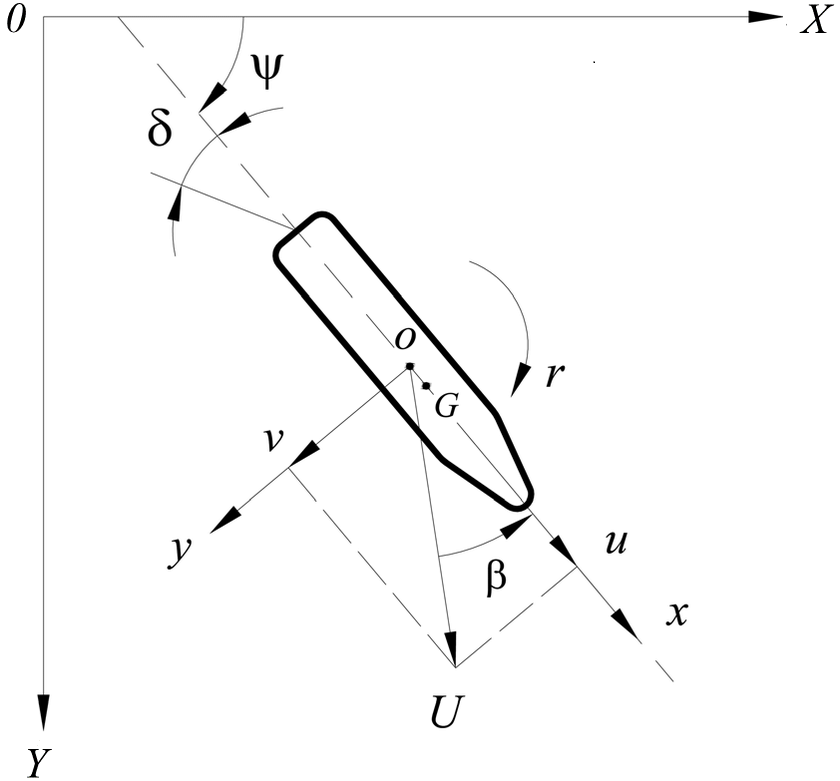
\includegraphics[width=0.48\linewidth]{Cxyz.png}
	% part in the [] goes to list of table, part in {} goes to text
	\caption[Space and ship-fixed coordinate system.]{Space and ship-fixed coordinate system. Adapted from \citet{luo2016parameter}.}
	\label{fig:cxyz}
\end{figure}
In the ship-fixed coordinate system, \textit{x} is pointing forward, \textit{y} to starboard and \textit{z} downwards. The origin of the space-fixed coordinate system is usually taken as lying on the undisturbed free surface.  A positive yaw angle $\psi$ is therefore defined as a \emph{clockwise} rotation of the ship in the space-fixed coordinate system. Similarly, a positive drift angle $\beta$ corresponds to the flow coming from starboard.

% input methodology
\chapter{Methodology}
Mauris pharetra et ultrices neque ornare aenean. Nascetur ridiculus mus mauris vitae ultricies. Placerat orci nulla pellentesque dignissim enim sit amet. Quis risus sed vulputate odio ut. Semper feugiat nibh sed pulvinar proin gravida hendrerit lectus. Nec feugiat nisl pretium fusce id velit ut tortor. Non quam lacus suspendisse faucibus interdum posuere lorem. Lorem sed risus ultricies tristique nulla. Non sodales neque sodales ut etiam sit amet. Sagittis purus sit amet volutpat consequat mauris nunc congue nisi.

\section{Section of Methodology}

Mauris pharetra et ultrices neque ornare aenean. Nascetur ridiculus mus mauris vitae ultricies. Placerat orci nulla pellentesque dignissim enim sit amet. Quis risus sed vulputate odio ut. Semper feugiat nibh sed pulvinar proin gravida hendrerit lectus. Nec feugiat nisl pretium fusce id velit ut tortor. Non quam lacus suspendisse faucibus interdum posuere lorem. Lorem sed risus ultricies tristique nulla. Non sodales neque sodales ut etiam sit amet. Sagittis purus sit amet volutpat consequat mauris nunc congue nisi. 

\subsection{Sub-section of Methodology}

Mauris pharetra et ultrices neque ornare aenean. Nascetur ridiculus mus mauris vitae ultricies. Placerat orci nulla pellentesque dignissim enim sit amet. Quis risus sed vulputate odio ut. Semper feugiat nibh sed pulvinar proin gravida hendrerit lectus. Nec feugiat nisl pretium fusce id velit ut tortor. Non quam lacus suspendisse faucibus interdum posuere lorem. Lorem sed risus ultricies tristique nulla. Non sodales neque sodales ut etiam sit amet. Sagittis purus sit amet volutpat consequat mauris nunc congue nisi.

\begin{figure}[]
	\centering
	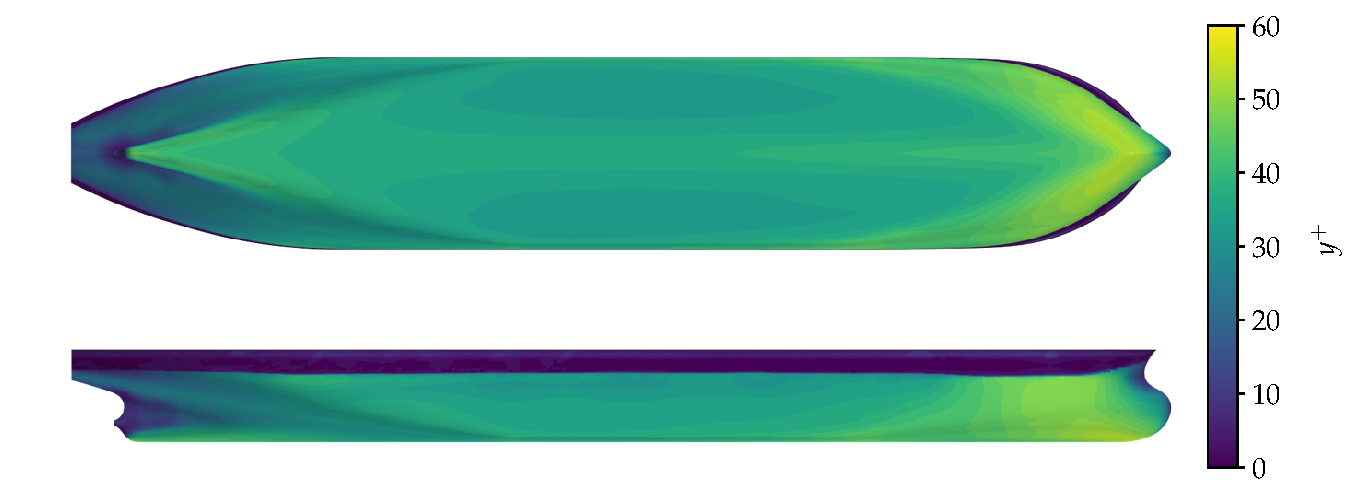
\includegraphics[width=1.0\linewidth]{yplus_0.pdf}  
	% part in the [] goes to list of table, part in {} goes to text 
	\caption{Bottom and profile view of the non-dimensional wall distance ($y^{+}$) on the KVLCC2 for the static drift simulation ($\beta=0^{\circ}$, $Fr=0.142$).}
	\label{fig:yplus}
\end{figure}
At quis risus sed vulputate. Amet risus nullam eget felis eget nunc. Ac felis donec et odio pellentesque. A iaculis at erat pellentesque adipiscing. A pellentesque sit amet porttitor. Ridiculus mus mauris vitae ultricies leo integer malesuada nunc vel. Cras semper auctor neque vitae tempus quam pellentesque. Aliquam sem fringilla ut morbi tincidunt augue interdum. Nam aliquam sem et tortor consequat id porta nibh venenatis. Nullam vehicula ipsum a arcu. Bibendum neque egestas congue quisque egestas. Quis enim lobortis scelerisque fermentum dui. Nibh ipsum consequat nisl vel pretium lectus quam id. Arcu dictum varius duis at consectetur lorem donec massa sapien. In est ante in nibh mauris. Placerat vestibulum lectus mauris ultrices eros. Sit amet aliquam id diam maecenas. Viverra vitae congue eu consequat ac. Consequat mauris nunc congue nisi vitae suscipit tellus mauris.


\begin{table}[h!]
\caption{Example of a threeparttable, useful for footnotes in tables.}
\label{tab:solver}
\centering
    \begin{threeparttable}
    	\begin{tabular}{llc}
			\toprule
			Boundary & Quantity & Value \\
			\midrule
			Inlet  & -Turbulence Intensity & 0.01 \\
				   & -Turbulent Viscosity Ratio & 10.0 \\
				   & -Velocity & Wave\tnote{1} \\
				   & -Volume Fraction & Wave\tnote{1}\\
			Outlet & -Turbulence Intensity & 0.01 \\
				   & -Turbulent Viscosity Ratio & 10.0 \\
				   & -Pressure & Wave\tnote{1} \\
				   & -Volume Fraction & Wave\tnote{1}\\
			Hull   & -Shear Stress & No-Slip\\
			Deck   & -Shear Stress & Slip\\
			Tank Walls  & -Shear Stress & Slip\\
			\bottomrule
		\end{tabular} 
    	\begin{tablenotes}
			\footnotesize
    		\item[1] Star-CCM$^{+}$ uses flat-water waves when using the VOF model to specify the velocity, hydrostatic pressure and volume fraction at the boundaries.
    	\end{tablenotes}
    \end{threeparttable}
\end{table}

% input chapterX
\chapter{Chapter X}
Lorem ipsum dolor sit amet, consectetur adipiscing elit, sed do eiusmod tempor incididunt ut labore et dolore magna aliqua. At erat pellentesque adipiscing commodo elit. Nibh ipsum consequat nisl vel pretium. Risus feugiat in ante metus dictum at tempor commodo. Faucibus scelerisque eleifend donec pretium vulputate. Elit scelerisque mauris pellentesque pulvinar. Aliquam etiam erat velit scelerisque in. In cursus turpis massa tincidunt dui. Turpis massa tincidunt dui ut ornare lectus sit. Lectus nulla at volutpat diam ut. Mauris augue neque gravida in fermentum et sollicitudin ac orci. Sit amet venenatis urna cursus eget nunc scelerisque viverra. Elit duis tristique sollicitudin nibh sit amet.

\section{Section of chapter X}

Lorem ipsum dolor sit amet, consectetur adipiscing elit, sed do eiusmod tempor incididunt ut labore et dolore magna aliqua. At erat pellentesque adipiscing commodo elit. Nibh ipsum consequat nisl vel pretium. Risus feugiat in ante metus dictum at tempor commodo. Faucibus scelerisque eleifend donec pretium vulputate. Elit scelerisque mauris pellentesque pulvinar. Aliquam etiam erat velit scelerisque in. In cursus turpis massa tincidunt dui. Turpis massa tincidunt dui ut ornare lectus sit. Lectus nulla at volutpat diam ut. Mauris augue neque gravida in fermentum et sollicitudin ac orci. Sit amet venenatis urna cursus eget nunc scelerisque viverra. Elit duis tristique sollicitudin nibh sit amet.

Viverra orci sagittis eu volutpat odio. Ac orci phasellus egestas tellus rutrum tellus. Accumsan in nisl nisi scelerisque eu. Ac tortor dignissim convallis aenean et tortor at risus. Amet nulla facilisi morbi tempus iaculis urna id volutpat. Nisl nunc mi ipsum faucibus vitae aliquet nec. Dolor purus non enim praesent elementum facilisis leo vel fringilla. Nunc scelerisque viverra mauris in aliquam sem fringilla. Arcu non sodales neque sodales ut etiam sit amet nisl. Vel orci porta non pulvinar neque laoreet suspendisse. Integer enim neque volutpat ac tincidunt. Imperdiet proin fermentum leo vel orci porta non. Molestie a iaculis at erat pellentesque adipiscing commodo elit. Blandit aliquam etiam erat velit scelerisque.

At quis risus sed vulputate. Amet risus nullam eget felis eget nunc. Ac felis donec et odio pellentesque. A iaculis at erat pellentesque adipiscing. A pellentesque sit amet porttitor. Ridiculus mus mauris vitae ultricies leo integer malesuada nunc vel. Cras semper auctor neque vitae tempus quam pellentesque. Aliquam sem fringilla ut morbi tincidunt augue interdum. Nam aliquam sem et tortor consequat id porta nibh venenatis. Nullam vehicula ipsum a arcu. Bibendum neque egestas congue quisque egestas. Quis enim lobortis scelerisque fermentum dui. Nibh ipsum consequat nisl vel pretium lectus quam id. Arcu dictum varius duis at consectetur lorem donec massa sapien. In est ante in nibh mauris. Placerat vestibulum lectus mauris ultrices eros. Sit amet aliquam id diam maecenas. Viverra vitae congue eu consequat ac. Consequat mauris nunc congue nisi vitae suscipit tellus mauris.

Sit amet tellus cras adipiscing enim eu. Nulla porttitor massa id neque aliquam vestibulum morbi blandit. Maecenas sed enim ut sem viverra. Eu volutpat odio facilisis mauris sit amet massa vitae. Pharetra magna ac placerat vestibulum lectus mauris. Scelerisque felis imperdiet proin fermentum leo vel orci porta non. Ullamcorper a lacus vestibulum sed arcu non. Sit amet massa vitae tortor. Odio ut enim blandit volutpat maecenas volutpat blandit. Gravida dictum fusce ut placerat orci nulla pellentesque dignissim enim. Integer eget aliquet nibh praesent tristique. Cursus vitae congue mauris rhoncus aenean vel elit scelerisque mauris. Viverra aliquet eget sit amet tellus.

Mauris pharetra et ultrices neque ornare aenean. Nascetur ridiculus mus mauris vitae ultricies. Placerat orci nulla pellentesque dignissim enim sit amet. Quis risus sed vulputate odio ut. Semper feugiat nibh sed pulvinar proin gravida hendrerit lectus. Nec feugiat nisl pretium fusce id velit ut tortor. Non quam lacus suspendisse faucibus interdum posuere lorem. Lorem sed risus ultricies tristique nulla. Non sodales neque sodales ut etiam sit amet. Sagittis purus sit amet volutpat consequat mauris nunc congue nisi.

% input chapterXX
\chapter{Chapter XX}
Lorem ipsum dolor sit amet, consectetur adipiscing elit, sed do eiusmod tempor incididunt ut labore et dolore magna aliqua. At erat pellentesque adipiscing commodo elit. Nibh ipsum consequat nisl vel pretium. Risus feugiat in ante metus dictum at tempor commodo. Faucibus scelerisque eleifend donec pretium vulputate. Elit scelerisque mauris pellentesque pulvinar. Aliquam etiam erat velit scelerisque in. In cursus turpis massa tincidunt dui. Turpis massa tincidunt dui ut ornare lectus sit. Lectus nulla at volutpat diam ut. Mauris augue neque gravida in fermentum et sollicitudin ac orci. Sit amet venenatis urna cursus eget nunc scelerisque viverra. Elit duis tristique sollicitudin nibh sit amet.

Sit amet tellus cras adipiscing enim eu. Nulla porttitor massa id neque aliquam vestibulum morbi blandit. Maecenas sed enim ut sem viverra. Eu volutpat odio facilisis mauris sit amet massa vitae. Pharetra magna ac placerat vestibulum lectus mauris. Scelerisque felis imperdiet proin fermentum leo vel orci porta non. Ullamcorper a lacus vestibulum sed arcu non. Sit amet massa vitae tortor. Odio ut enim blandit volutpat maecenas volutpat blandit. Gravida dictum fusce ut placerat orci nulla pellentesque dignissim enim. Integer eget aliquet nibh praesent tristique. Cursus vitae congue mauris rhoncus aenean vel elit scelerisque mauris. Viverra aliquet eget sit amet tellus.

Mauris pharetra et ultrices neque ornare aenean. Nascetur ridiculus mus mauris vitae ultricies. Placerat orci nulla pellentesque dignissim enim sit amet. Quis risus sed vulputate odio ut. Semper feugiat nibh sed pulvinar proin gravida hendrerit lectus. Nec feugiat nisl pretium fusce id velit ut tortor. Non quam lacus suspendisse faucibus interdum posuere lorem. Lorem sed risus ultricies tristique nulla. Non sodales neque sodales ut etiam sit amet. Sagittis purus sit amet volutpat consequat mauris nunc congue nisi.

\begin{table}
\caption{Another threeparttable example.}
\label{tab:gci}
\centering
    \begin{threeparttable}
    	\begin{tabular}{cccc}
			\toprule
			 & $X$ (N)  & $Y$ (N) & $N$ (Nm) \\
			\midrule
			$\hat{S}_{k1}$ (Fine) & -3.111 & 5.512 & 8.860 \\
			$\hat{S}_{k2}$ (Standard) & -3.094 & 5.502 & 8.8544 \\
			$\hat{S}_{k3}$ (Coarse) & -3.065 & 5.483 & 8.8540 \\
			Convergence\tnote{1} & M & M & M \\
			\textbf{\textit{p}} (apparent order) & \textbf{3.31} & \textbf{4.13} & \textbf{12.13} \\
			$\hat{S}_{\text{ext}}^{21}$ & -3.129 & 5.519 & 8.861 \\
			$e_{\text{a}}^{21}$ & 0.55 & 0.18 & 0.07 \\
			$e_{\text{ext}}^{21}$ & 0.56 & 0.14 & 0.01 \\
			$\textbf{GCI}_{\text{standard}}^{21}$ & \textbf{1.41} & \textbf{0.4} & \textbf{0.0074} \\
			\bottomrule
		\end{tabular} 
    	\begin{tablenotes}
			\footnotesize
    		\item[1] M: monotonic convergence, O: oscillatory convergence, D: divergence 
    	\end{tablenotes}
    \end{threeparttable}
\end{table}

% input conclusion
\chapter{Conclusion and Future Work}
Lorem ipsum dolor sit amet, consectetur adipiscing elit, sed do eiusmod tempor incididunt ut labore et dolore magna aliqua. At erat pellentesque adipiscing commodo elit. Nibh ipsum consequat nisl vel pretium. Risus feugiat in ante metus dictum at tempor commodo. 

\section{Conclusions}

RLorem ipsum dolor sit amet, consectetur adipiscing elit, sed do eiusmod tempor incididunt ut labore et dolore magna aliqua. At erat pellentesque adipiscing commodo elit. Nibh ipsum consequat nisl vel pretium. Risus feugiat in ante metus dictum at tempor commodo. Faucibus scelerisque eleifend donec pretium vulputate. Elit scelerisque mauris pellentesque pulvinar. Aliquam etiam erat velit scelerisque in. In cursus turpis massa tincidunt dui. Turpis massa tincidunt dui ut ornare lectus sit. Lectus nulla at volutpat diam ut. Mauris augue neque gravida in fermentum et sollicitudin ac orci. Sit amet venenatis urna cursus eget nunc scelerisque viverra. Elit duis tristique sollicitudin nibh sit amet.


At quis risus sed vulputate. Amet risus nullam eget felis eget nunc. Ac felis donec et odio pellentesque. A iaculis at erat pellentesque adipiscing. A pellentesque sit amet porttitor. Ridiculus mus mauris vitae ultricies leo integer malesuada nunc vel. Cras semper auctor neque vitae tempus quam pellentesque. Aliquam sem fringilla ut morbi tincidunt augue interdum. Nam aliquam sem et tortor consequat id porta nibh venenatis. Nullam vehicula ipsum a arcu. Bibendum neque egestas congue quisque egestas. Quis enim lobortis scelerisque fermentum dui. Nibh ipsum consequat nisl vel pretium lectus quam id. Arcu dictum varius duis at consectetur lorem donec massa sapien. In est ante in nibh mauris. Placerat vestibulum lectus mauris ultrices eros. Sit amet aliquam id diam maecenas. Viverra vitae congue eu consequat ac. Consequat mauris nunc congue nisi vitae suscipit tellus mauris.

\section{Recommendations for Future Work}

Sit amet tellus cras adipiscing enim eu. Nulla porttitor massa id neque aliquam vestibulum morbi blandit. Maecenas sed enim ut sem viverra. Eu volutpat odio facilisis mauris sit amet massa vitae. Pharetra magna ac placerat vestibulum lectus mauris. Scelerisque felis imperdiet proin fermentum leo vel orci porta non. Ullamcorper a lacus vestibulum sed arcu non. Sit amet massa vitae tortor. Odio ut enim blandit volutpat maecenas volutpat blandit. Gravida dictum fusce ut placerat orci nulla pellentesque dignissim enim. Integer eget aliquet nibh praesent tristique. Cursus vitae congue mauris rhoncus aenean vel elit scelerisque mauris. Viverra aliquet eget sit amet tellus.

Mauris pharetra et ultrices neque ornare aenean. Nascetur ridiculus mus mauris vitae ultricies. Placerat orci nulla pellentesque dignissim enim sit amet. Quis risus sed vulputate odio ut. Semper feugiat nibh sed pulvinar proin gravida hendrerit lectus. Nec feugiat nisl pretium fusce id velit ut tortor. Non quam lacus suspendisse faucibus interdum posuere lorem. Lorem sed risus ultricies tristique nulla. Non sodales neque sodales ut etiam sit amet. Sagittis purus sit amet volutpat consequat mauris nunc congue nisi.







% create phantom section for REFERENCES, with link in table of content
\newpage
\phantomsection 
\addcontentsline{toc}{chapter}{References} 
\printbibliography[title={References}]

% input as appendix
\appendix
\chapter{Writing Equations}

The following present the details of the different turbulence closure models used. For a complete explanation of the implementation of the different models, refer to \citet{starccm}.

\section{Different Equations}
Menter's formulation of the $k$-$\omega$ turbulence model is used \citep{menter1994two}, where the turbulent kinematic energy $k$ is given by
\begin{equation}
\frac{Dk}{Dt}=\tau_{ij}\frac{\partial u_{i}}{\partial x_{j}}-\beta^{\star}\rho\omega k+\frac{\partial}{\partial x_{j}}\left[(\mu+\sigma_{k1}\mu_{t})\frac{\partial k}{\partial x_{j}}\right] \,,
\end{equation}
and the specific dissipation rate $\omega$,
\begin{equation}
\begin{split}
\frac{D\rho\omega}{Dt} & =\frac{\gamma}{\nu_{t}}\tau_{ij}\frac{\partial u_{i}}{\partial x_{j}}-\beta\rho\omega^{2}+\frac{\partial}{\partial x_{j}}\left[(\mu+\sigma_{\omega}\mu_{t})\frac{\partial\omega}{\partial x_{j}}\right] \\
& +2\rho(1-F_{1})\sigma_{\omega 2}\frac{1}{\omega}\frac{\partial k}{\partial x_{j}}\frac{\partial\omega}{\partial x_{j}} \,.
\end{split}
\end{equation}
$F_{1}$ is a blending function that calculates the new model constants $\phi$ from the constant $\phi_{1}$ and $\phi_{2}$,
\begin{equation}
\phi=F_{1}\phi_{1}+(1-F_{1})\phi_{2} \,.
\end{equation}
The turbulent viscosity is calculated using the turbulent kinetic energy and the specific dissipation rate
\begin{equation}
\nu_{t}=\frac{a_{1}k}{\max(a_{1}\omega;\Omega F_{2})} \,,
\end{equation}
with
\begin{equation}
F_2=\tanh(arg_{2}^{2}) \,,
\end{equation}
where,
\begin{equation}
arg_{2}=max\left(2\frac{\sqrt{k}}{0.09\omega y};\frac{500\nu}{y^2 \omega}\right)  \,.
\end{equation}
The constant of set $\phi_{1}$ are (SST inner):
\begin{table}[H]
\centering
	\begin{tabular}{ccccc}
	$\kappa$ = 0.41 & $\beta^{\star}$ = 0.09 & $\beta_{1}$ = 0.0750 & $\sigma_{k1}$ = 0.85 \\ 
	$\sigma_{\omega 1}$ = 0.5 & $a_{1}$ = 0.31 &  \multicolumn{2}{c}{$\gamma_{1}=\beta_{1}/\beta^{\star}-\sigma_{\omega 1}\kappa^{2}/\sqrt{\beta^{\star}}$} \\
	\end{tabular}
\end{table}
\noindent
The constant of set $\phi_{2}$ are (standard $k$-$\epsilon$):
\begin{table}[H]
\centering
	\begin{tabular}{ccccc}
	$\kappa$ = 0.41 & $\beta^{\star}$ = 0.09 & $\beta_{2}$ = 0.0828 & $\sigma_{k2}$ = 1.0 \\ 
	$\sigma_{\omega 2}$ = 0.856 &  \multicolumn{3}{c}{$\gamma_{2}=\beta_{2}/\beta^{\star}-\sigma_{\omega 2}\kappa^{2}/\sqrt{\beta^{\star}}$} \\
	\end{tabular}
\end{table}

\chapter{Other Tricks}

\section{Standard appendix}
Boundary layer theory can be used to determine the required first cell height and the depth of the boundary layer for meshing. First the Reynolds number of the simulation is determined, using fresh water properties
\begin{equation} 
	Re_{x}=\frac{Ux}{\nu}=\frac{0.76\cdot2.9091}{1.138\times10^{-6}}=1.94\times10^{6} \,.
\end{equation}
The wall distance can be calculated using the ITTC skin-friction correlation line
\begin{equation}
	C_f = \frac{0.075}{(\log(Re_x)-2)^2}=\frac{0.075}{(\log(1.94\times10^{6})-2)^2}=4.078\times10^{-3} \,,
\end{equation} 
for $Re_x < 10^9$. The wall shear stress can be expressed as
\begin{equation}
\tau_{w} = \frac{1}{2}\rho U^2C_f  = \frac{1}{2}\cdot 999.1026 \cdot 0.76^{2}\cdot4.078\times10^{-3}= 1.176 \,.
\end{equation}
From this the friction velocity can be calculated
\begin{equation}
u_{*} = \sqrt{\frac{\tau_{w}}{\rho}} = \sqrt{\frac{1.176}{9989.1026}}=0.0343 \,.
\end{equation}
And finally, the wall distance
\begin{equation}
y = \frac{y^{+}\nu}{u_{*}}=\frac{30\cdot 1.0034\times10^{-6} }{0.0343}= 0.000994 m \,.
\end{equation}
With a target y+ $\sim30$ the required first cell height is (this gives us the position of the first node, which is at the centre of the cell)
\begin{equation}
y=0.00198 m \,\,\sim \,\,2 mm \,.
\end{equation}
The total boundary layer depth can be estimated using Schilchting formula for a turbulent boundary layer over a flat plate \citep{schlichting1979boundary}
\begin{equation}
\frac{\delta}{x}=0.37Re_{x}^{-1/5}=0.37\cdot{1.94\times10^{6}}^{-1/5}= 0.02044 \,.
\end{equation}
At the stern, the boundary layer depth will be
\begin{equation}
\delta = 0.02044\cdot 2.9091 = 0.0595 m \,.
\end{equation}


\section{Include code (Python and more)}
\begin{lstlisting}[language=Python]
from scipy.signal import butter, filtfilt

# Filter for experimental data
def butter_lowpass(cutoff, fs, order):
    nyq = 0.5 * fs
    normal_cutoff = cutoff / nyq
    b, a = butter(order, normal_cutoff, btype='low', analog=False)
    return b, a

def butter_lowpass_filter(data, cutoff, fs, order):
    b, a = butter_lowpass(cutoff, fs, order=order)
    y = filtfilt(b, a, data)					
    return y
\end{lstlisting}


% last page LEFT BLANK INTENTIONALLY
\newpage
	\begin{center}
	\thispagestyle{empty}
	\vspace*{\fill}
	Page left intentionally blank.
	\vspace*{\fill}
	\end{center}
\newpage

\end{document}